\documentclass{article}
\usepackage[margin=1in]{geometry}
\usepackage{graphicx}
\usepackage{pdfpages}
\usepackage{hyperref}
\hypersetup{
    colorlinks=true,
    linkcolor=blue,
    filecolor=magenta,      
    urlcolor=cyan,
}
\usepackage{float}
\usepackage{caption}
\usepackage{subcaption}
\usepackage{array}
\usepackage{enumitem}

\title{CS M152A Lab 4: Finite State Machine - Parking Meter}
\author{Arnold Pfahnl \\ \small{TA: Mohit Garg, Winter 2021}}
\date{}

% \begin{figure}[H]
%     \centering
%     \includegraphics[scale=0.44]{../figs/.png}
%     \caption{}
%     \label{fig:}
% \end{figure}

\begin{document}
\maketitle
\tableofcontents

\section{Introduction}
In this lab we utilize a finite state machine (FSM) to create a parking meter encapsulated by the Verilog module, $parking\_meter$. The functionality of this parking machine module includes simulating the ability to load coins and displaying the appropriate time remaining to four seven-segment LED displays. The required inputs are shown in Table \ref{table:inputs} below.

\begin{table}[H]
    \centering
    \begin{tabular}{ | c | c | }
        \hline
        \textbf{Inputs} & \textbf{Function}\\
        \hline
        $add1$ & Add 60 seconds. \\
        \hline
        $add2$ & Add 120 seconds. \\
        \hline
        $add3$ & Add 180 seconds. \\
        \hline
        $add4$ & Add 300 seconds. \\
        \hline
        $rst1$ & Reset time to 16 seconds. \\
        \hline
        $rst2$ & Reset time to 150 seconds. \\
        \hline
        $clk$ & 100 Hz system clock. \\
        \hline
        $rst$ & Resets to initial state.\\
        \hline
    \end{tabular}
    \caption{Inputs to $parking\_meter$ module. Each add and reset button is high for at most one clock cycle.}
    \label{table:inputs}
\end{table}

The output module has a seven-segment vector $led\_seg$ that displays the actual value fed to the four segments corresponding to the digits being displayed. Each segment in the vector represents CA, CB, CC, CD, CE, CF, and CG in Figure \ref{fig:four-7-seg}. Additionally, $a1$, $a2$, $a3$, and $a4$ are one-bit anodes that act as enables for their corresponding digits. As a form of redundancy, $val1$, $val2$, $val3$, and $val4$ are each four-bit output ports that display their corresponding digit in binary coded decimal (BCD).

\begin{figure}[H]
    \centering
    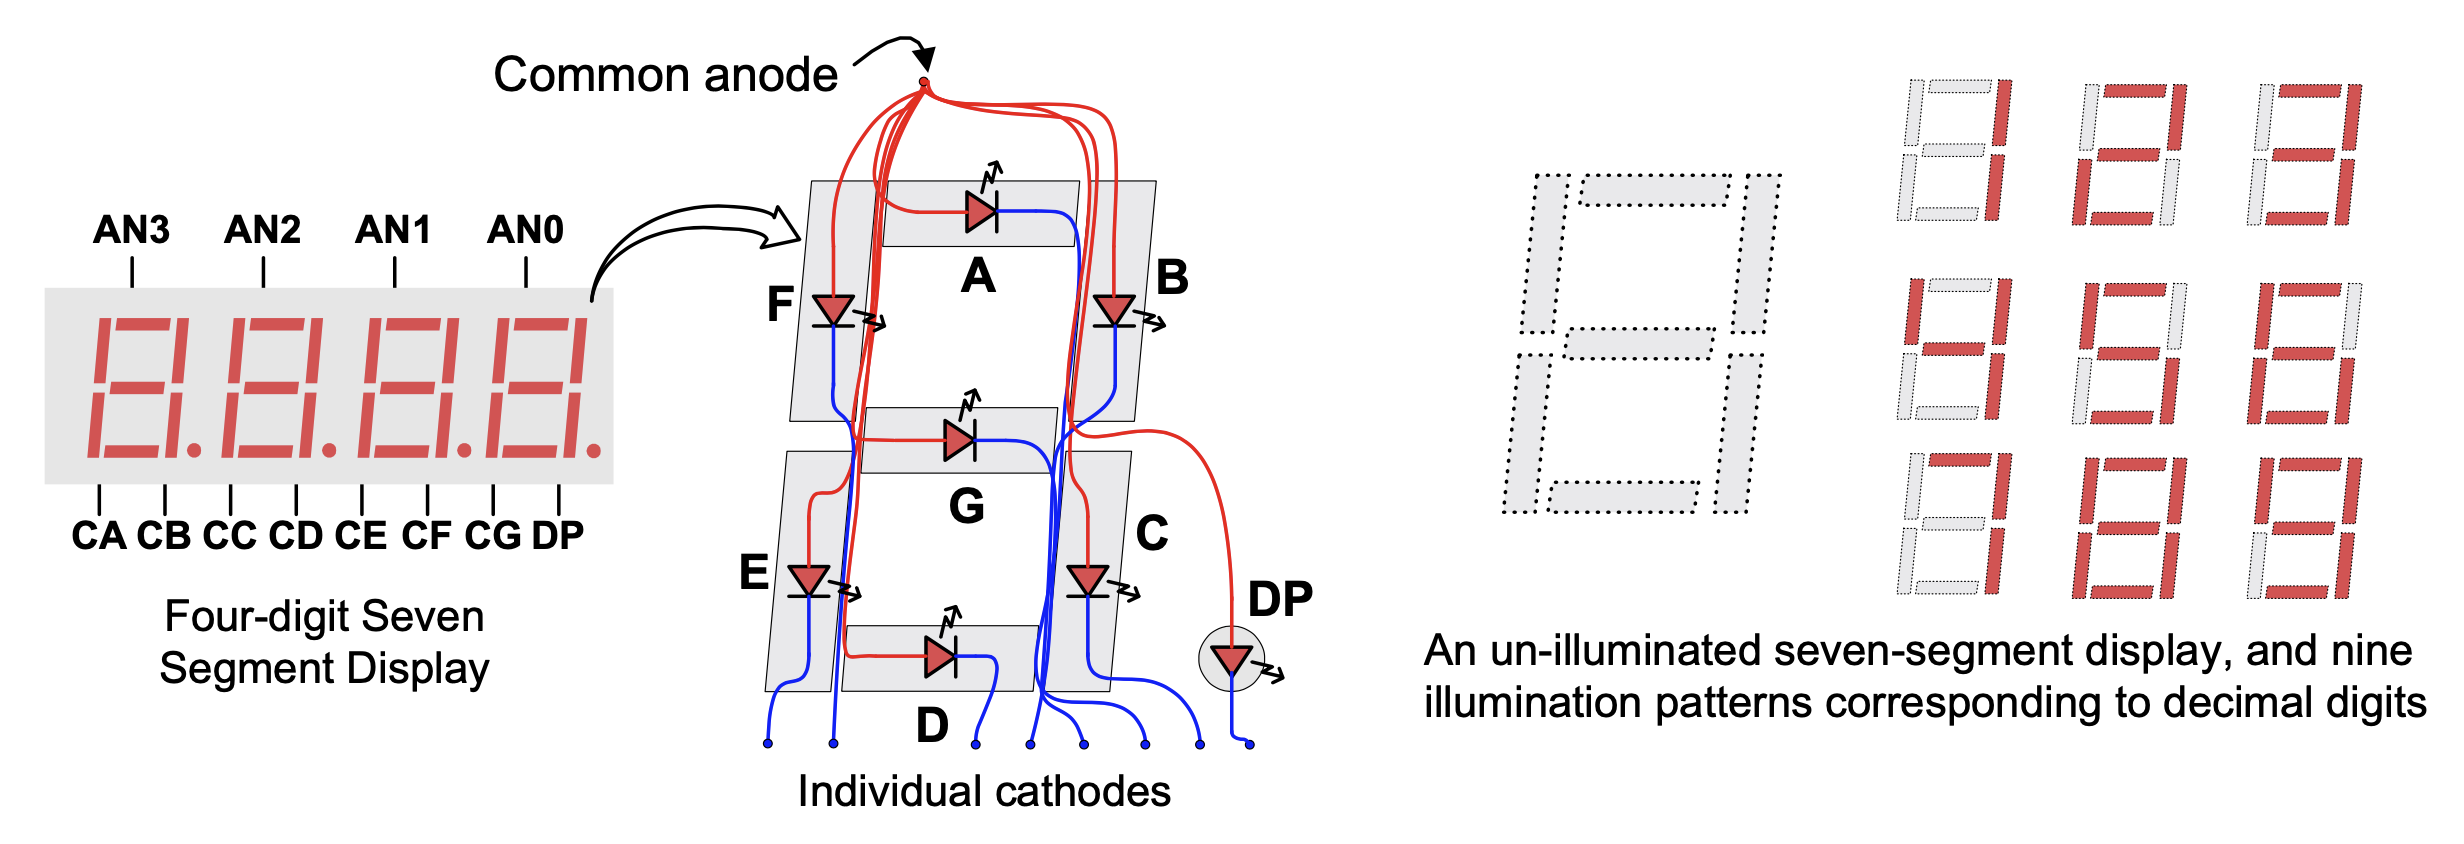
\includegraphics[scale=0.35]{../figs/four-7-seg.png}
    \caption{The four-digit seven-segment display specification for the Nexys3 board from Diligent Doc: 502-182.}
    \label{fig:four-7-seg}
\end{figure}

\section{Parking Meter Design}
The states of the parking meter are based on the FSM diagram in Figure \ref{fig:fsm}. An internal register called $counter$ stores the countdown. The three main states are INITIAL, ONE, and TWO:
\begin{enumerate}
    \item The \textbf{INITIAL} state flashes 0000 on the four seven-segment displays with a period of 1 second and duty cycle 50\%. If the $add4$ signal goes high, the machine enters the ONE state. If any other $add$ state goes high, the machine enters the TWO state. If $rst$ goes high, the machine will enter this state regardless of any other condition.
    \item The \textbf{ONE} state flashes the four-digit integer value of the $counter$ register with a period of 1 second and 50\% duty cycle. Once the value of $counter$ drops under 180, the machine will enter state TWO. If $rst1$ or $rst2$ are enabled, the machine will enter this state.
    \item The \textbf{TWO} state flashes the four-digit integer value of the $counter$ register with a period of 2 seconds and 50\% duty cycle. If the value of $counter$ is ever greater or equal to 180 due to an $add$, the machine will enter the ONE state. If the time expires ($counter$ is 0), then the machine loops back to the INITIAL state.
\end{enumerate}

Note that the machine does not account for multiple inputs being pressed at the same time.

\begin{figure}[H]
    \centering
    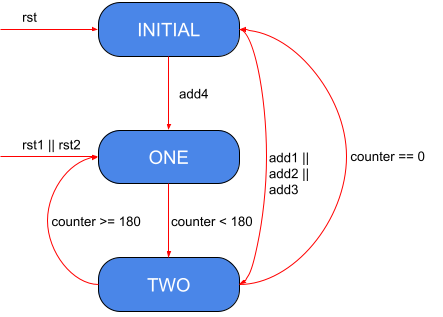
\includegraphics[scale=0.6]{../figs/FSM.png}
    \caption{Finite state machine (FSM) diagram for the $parking\_meter$ module.}
    \label{fig:fsm}
\end{figure}

To show a four-digit number, the Nexys3 reference recommends a scanning display controller. The anode signals and cathode patterns of each digit are driven in a repeating, continuous succession. This pattern is visualized in Figure \ref{fig:sig-action}.

\begin{figure}[H]
    \centering
    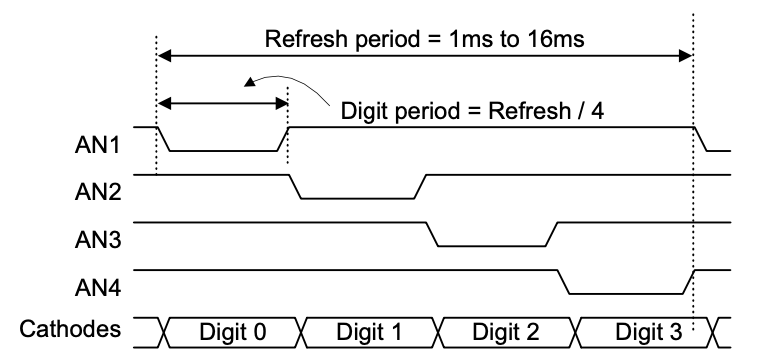
\includegraphics[scale=0.6]{../figs/sig-action.png}
    \caption{Four-digit display signal action for the Nexys3 board from Diligent Doc: 502-182.}
    \label{fig:sig-action}
\end{figure}

In my implementation an internal register $digI$ is set to the digit to be illuminated every one clock cycle. $digI$ begins at $0$, increments by one up to $3$ and then resets to $0$. A case statement then checks $digI$ to route the appropriate logic for setting the digit cathode and anode variables. Since each digit gets one cycle in my implementation, it takes 4 input cycles to get through all digits making the overall cycle 25 Hz.

I also have two internal registers $fast\_cycle$ and $slow\_cycle$ that count up to 100 and 200 respectively and act as pseudo-clocks. To flash for a period of one second and a duty cycle of 50\%, I display the values up until $fast\_cycle$ reaches 50 and then stop displaying until the next time $fast\_cycle$ loops back to 0. The same logic applies for flashing for a period of two seconds and 50\% duty cycle, just with $slow\_cycle$.

\pagebreak
\subsection{Schematics}
The top level schematic in Figure \ref{fig:schem_top} hides the considerable complexity of the RTL schematic in Figure \ref{fig:schem_detailed}. Due to the combination of both combinational and sequential logic used to determine states and output, the RTL features a mess of registers, muxes, and many other gates.
\begin{figure}[H]
    \centering
    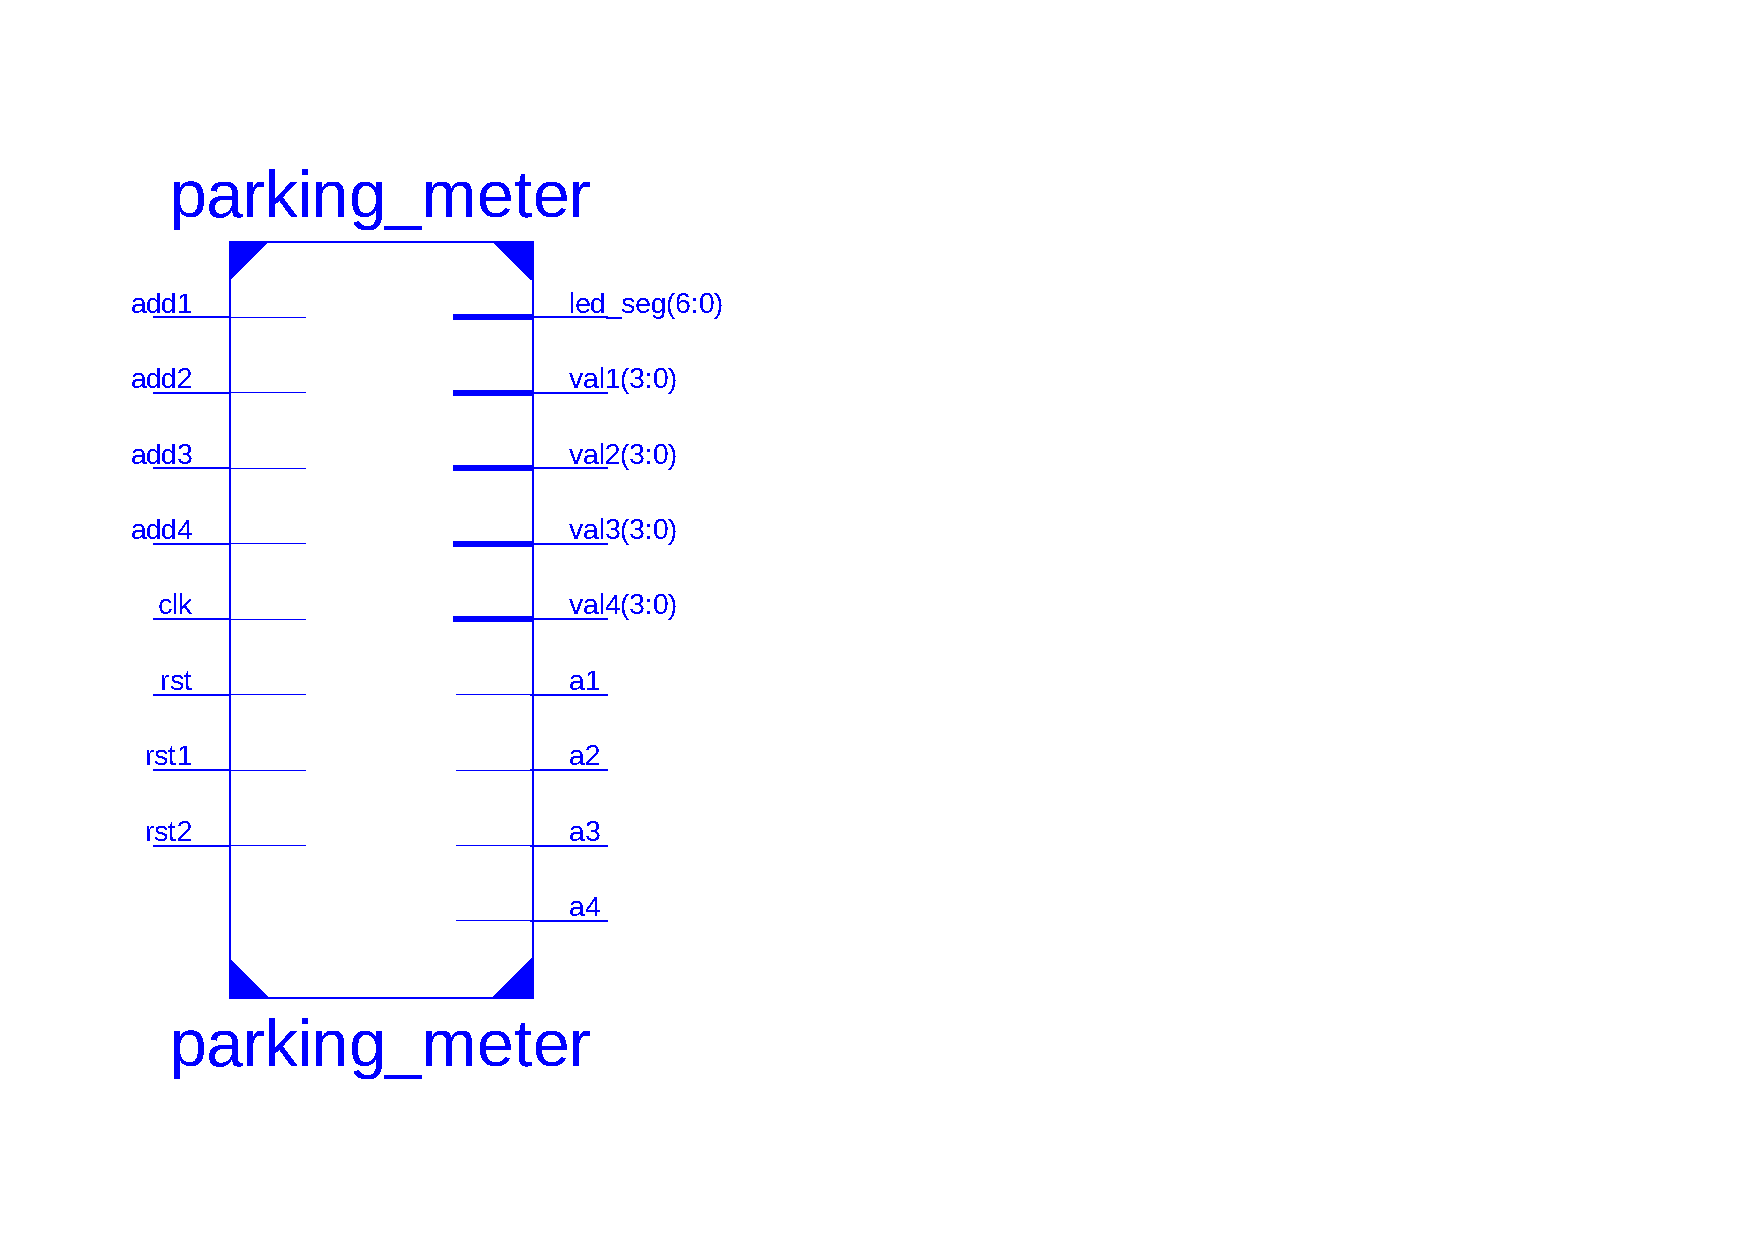
\includegraphics[scale=0.42]{../figs/rtl-top.pdf}
    \caption{Top level schematic for the $parking\_meter$ module.}
    \label{fig:schem_top}
\end{figure}

\begin{figure}[H]
    \centering
    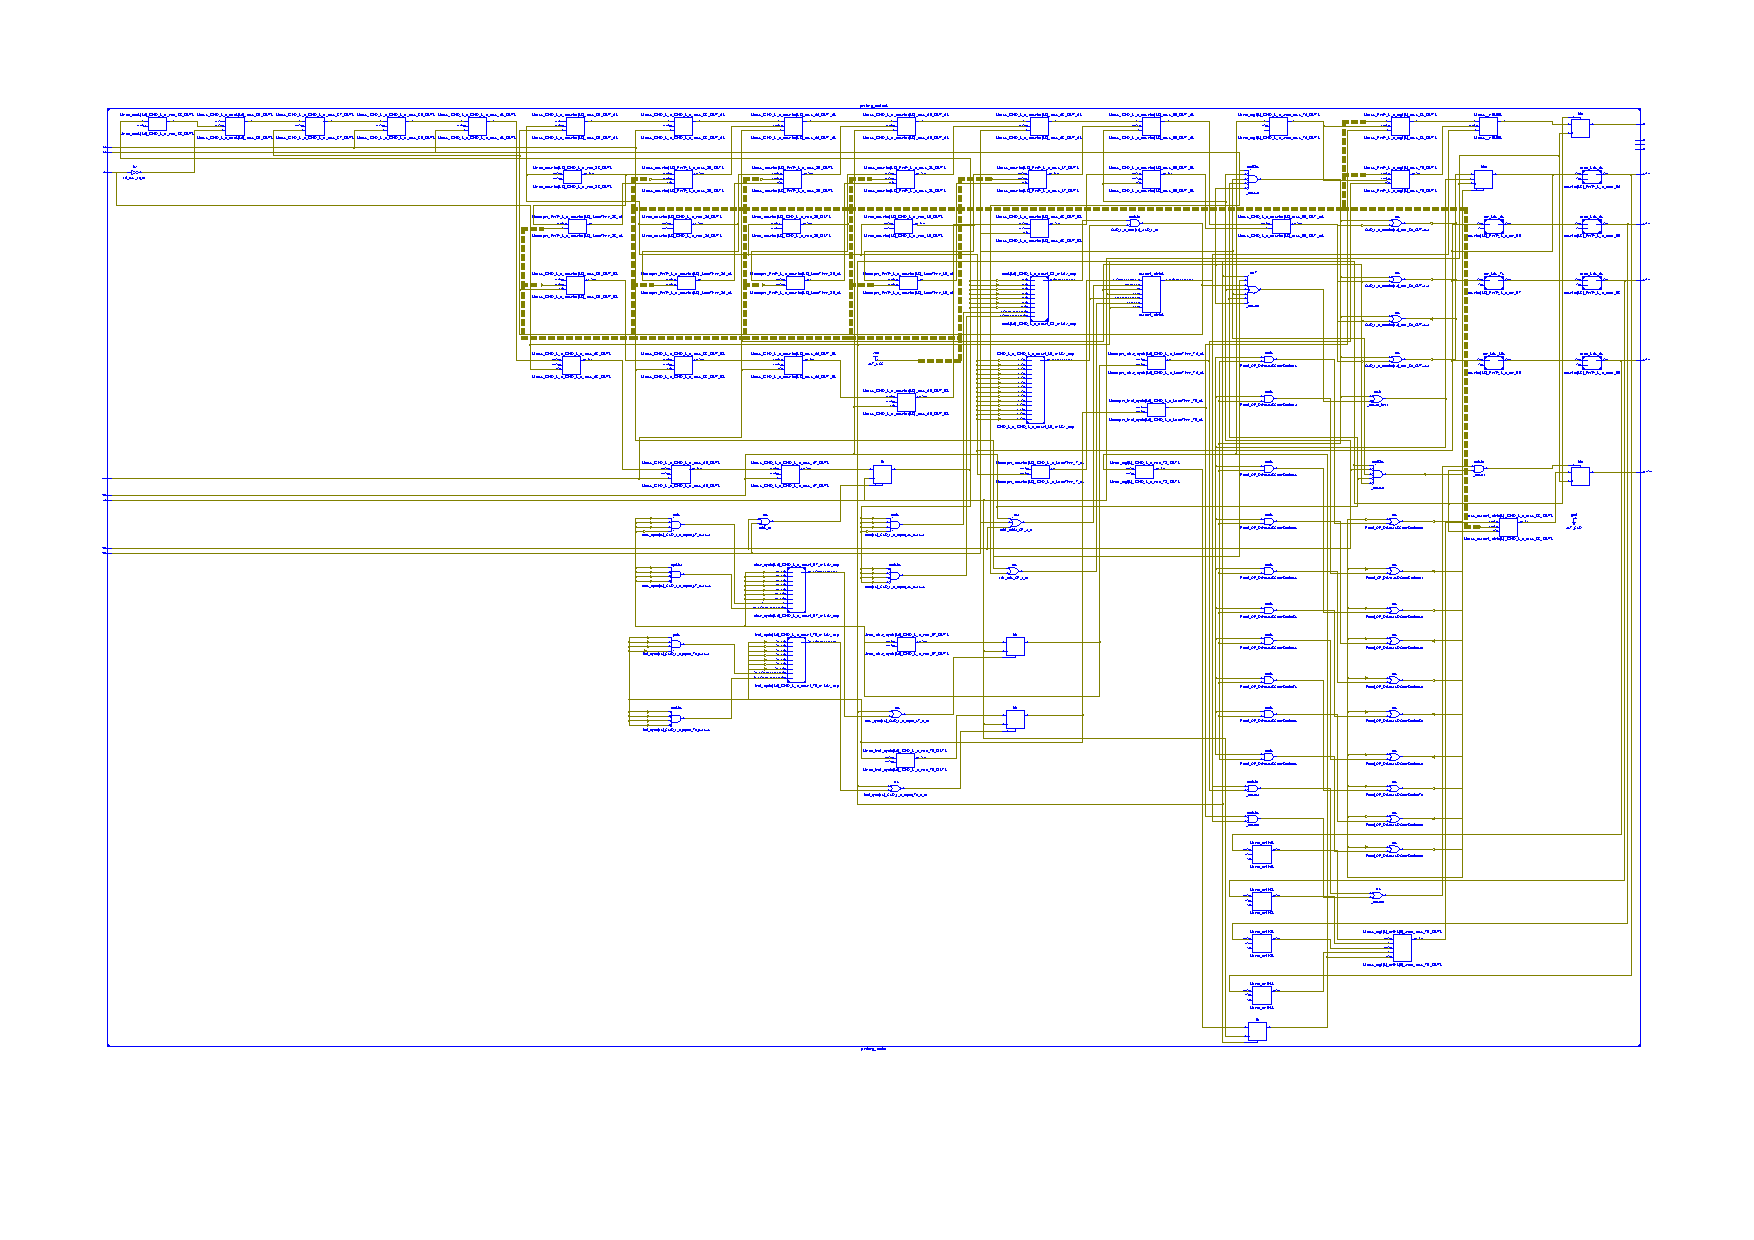
\includegraphics[scale=0.6]{../figs/rtl-low.pdf}
    \caption{Detailed RTL schematic for the $parking\_meter$ module.}
    \label{fig:schem_detailed}
\end{figure}

\subsection{Design Summary Report}

{\centering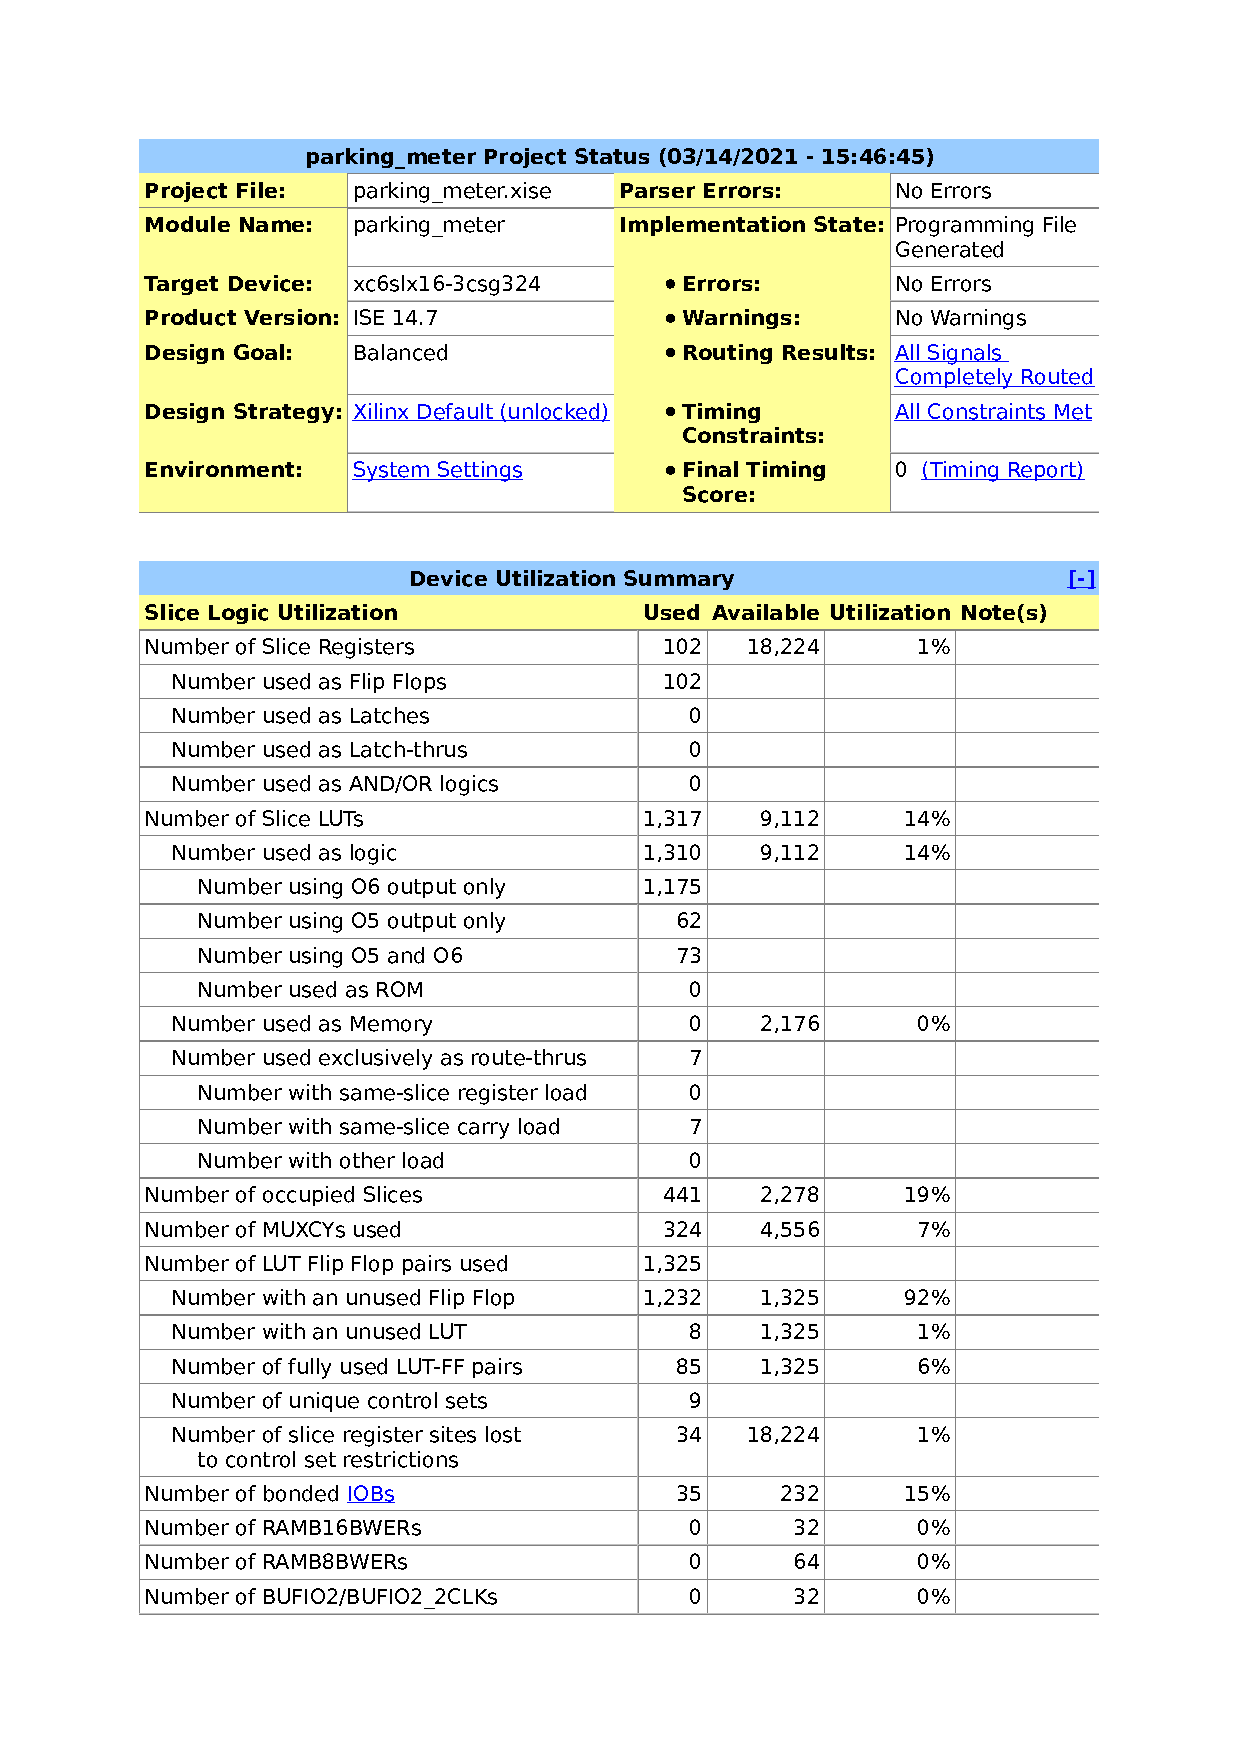
\includegraphics[scale=0.8, page=1]{../figs/summary.pdf}\par}

{\centering\includegraphics[scale=0.8, page=2]{../figs/summary.pdf}\par}

{\centering\includegraphics[scale=0.8, page=3]{../figs/summary.pdf}\par}

\pagebreak
\section{Simulation}
The following test cases encompass all possible functions of the parking meter in addition to some corner cases.
\begin{enumerate}
    \item \textbf{Add 60 seconds.} This test encompasses many base cases including making sure that the INITIAL state flashing is working, the TWO state flashing is working properly, global reset works, adding works, and that the countdown is working. There were no issues with this test case.
        \begin{figure}[H]
            \centering
            \begin{subfigure}{\textwidth}
                \centering
                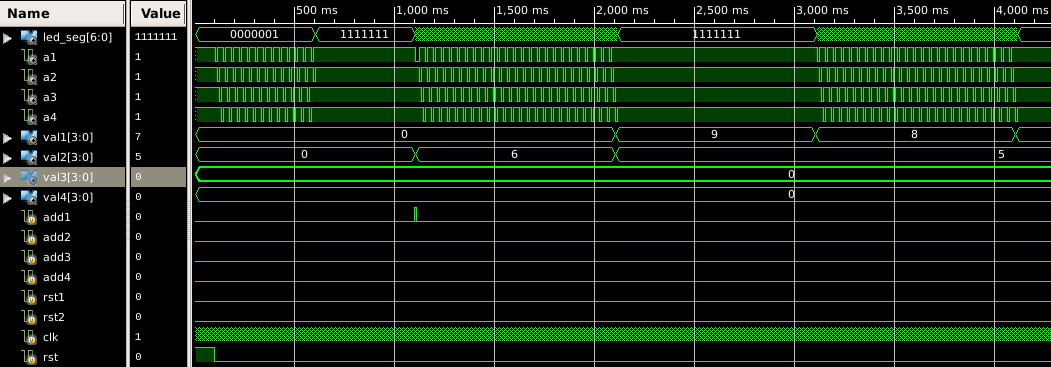
\includegraphics[scale=0.34]{../figs/add60-m.png}
                \caption{Initial countdown after adding 60 seconds.}
            \end{subfigure}
            \begin{subfigure}{\textwidth}
                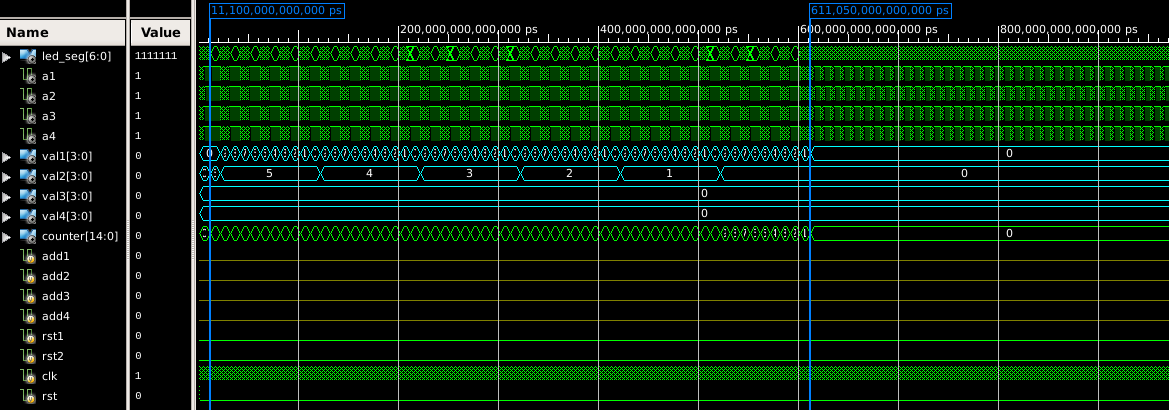
\includegraphics[scale=0.4]{../figs/add60-l.png}
                \caption{Full 60 second countdown.}
            \end{subfigure}
            \begin{subfigure}{\textwidth}
                \centering
                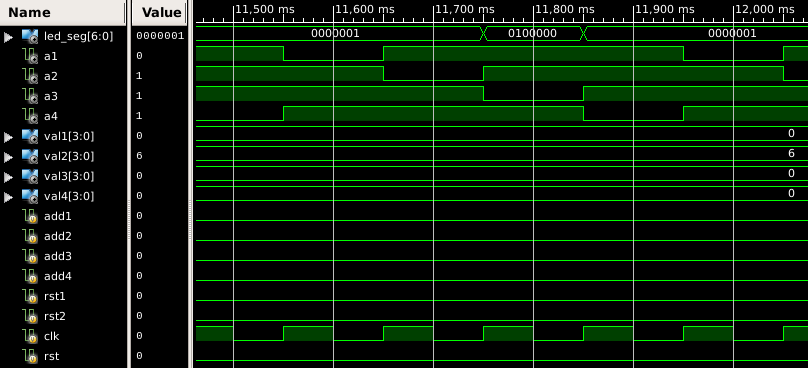
\includegraphics[scale=0.35]{../figs/add60-s.png}
                \caption{Zoomed in view with the scanning display values.}
            \end{subfigure}
            \caption{Different views of the 60 second addition waveform ($add1$ signal).}
            \label{fig:add1}
        \end{figure}
    \item \textbf{Add 120 seconds.} This test case is a continuation of the previous test case to make sure that $add2$ is working properly. This test case also had no issues.
        \begin{figure}[H]
            \centering
            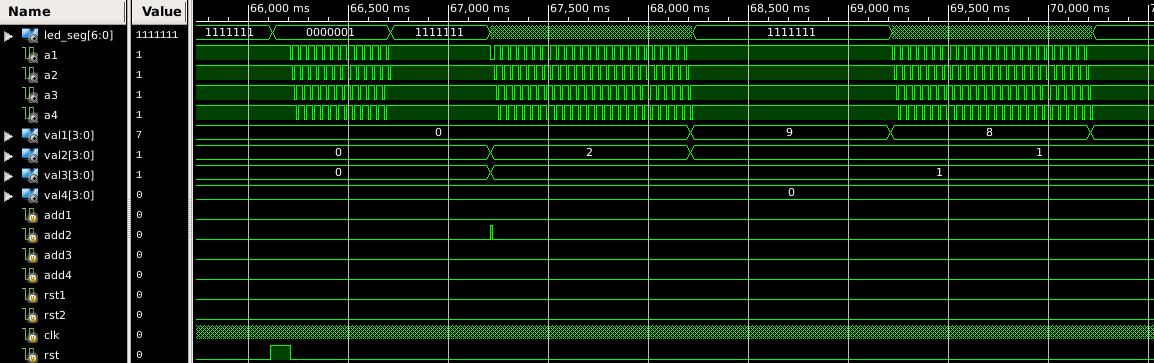
\includegraphics[scale=0.35]{../figs/add120.png}
            \caption{Testing the $add2$ signal.}
            \label{fig:add2}
        \end{figure}
    \item \textbf{Add 180 seconds.} Here I check that $add3$ is working properly. This test case passed with no issues.
        \begin{figure}[H]
            \centering
            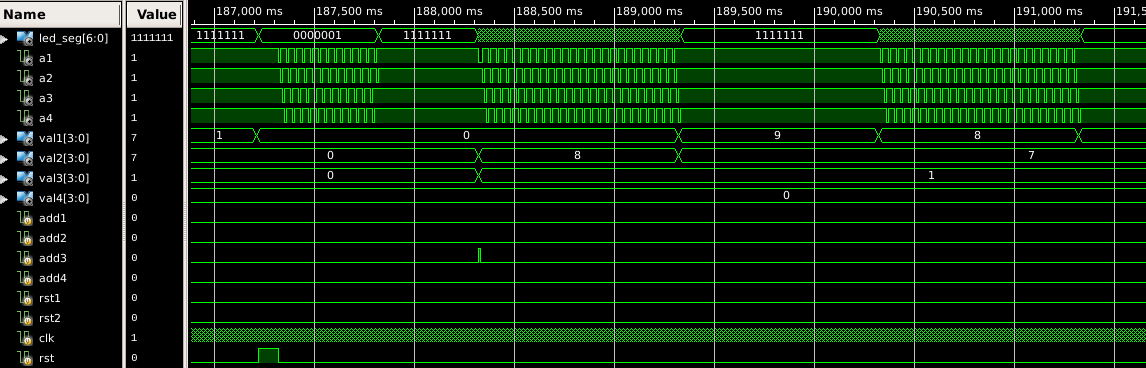
\includegraphics[scale=0.35]{../figs/add180.png}
            \caption{Testing the $add3$ signal.}
            \label{fig:add3}
        \end{figure}
    \item \textbf{Add 300 seconds.} Here I check to make sure that $add4$ enters the ONE state and transitions from the ONE to TWO state correctly. This test case passes as expected.
        \begin{figure}[H]
            \centering
            \begin{subfigure}{\textwidth}
                \centering
                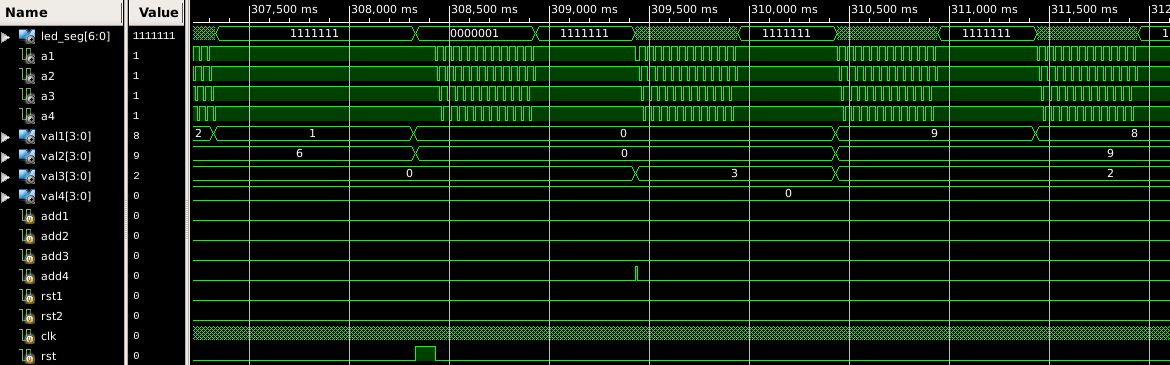
\includegraphics[scale=0.34]{../figs/add300-1.png}
                \caption{Initial countdown after adding 300 seconds. This section has a 1 second flash cycle.}
            \end{subfigure}
            \begin{subfigure}{\textwidth}
                \centering
                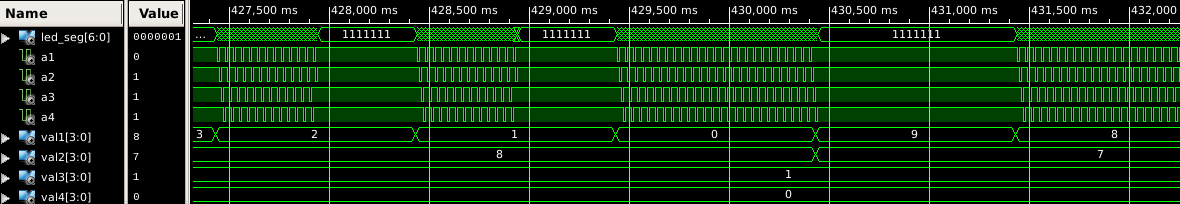
\includegraphics[scale=0.34]{../figs/add300-2.png}
                \caption{ONE to TWO state transition. 180 seconds and lower have a 2 second flash cycle.}
            \end{subfigure}
            \caption{$add3$ signal test case waveforms.}
            \label{fig:add4}
        \end{figure}
    \item \textbf{Add 300, reset time to 16 seconds, then reset time to 150 seconds.} Here I check that $rst1$ and $rst2$ work and that the transition from ONE to TWO state is working. This test passes as expected.
        \begin{figure}[H]
            \centering
            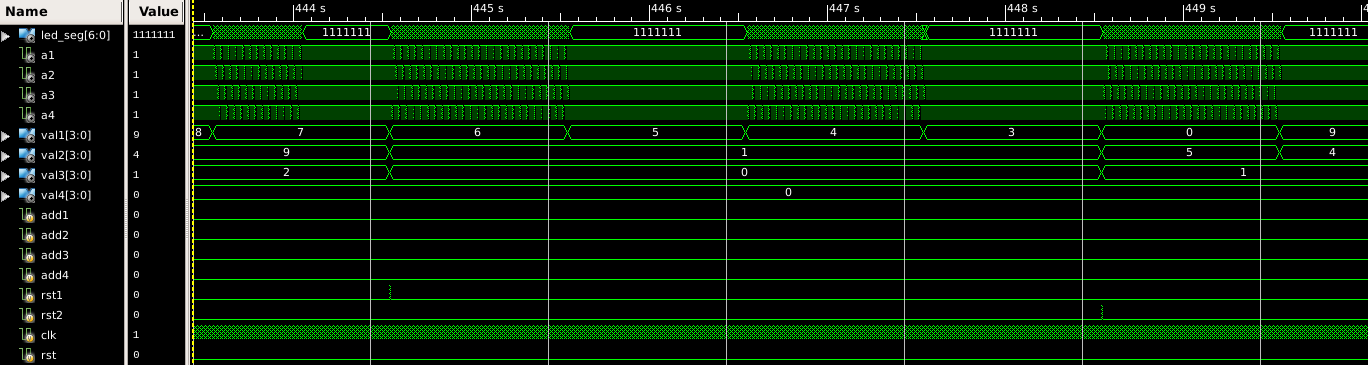
\includegraphics[scale=0.35]{../figs/rst.png}
            \caption{Testing $rst1$ and $rst2$.}
            \label{fig:rst}
        \end{figure}
    \item \textbf{Add beyond 9999 seconds.} Here I check that the counter doesn't exceed the maximum allowed value. This works as expected.
        \begin{figure}[H]
            \centering
            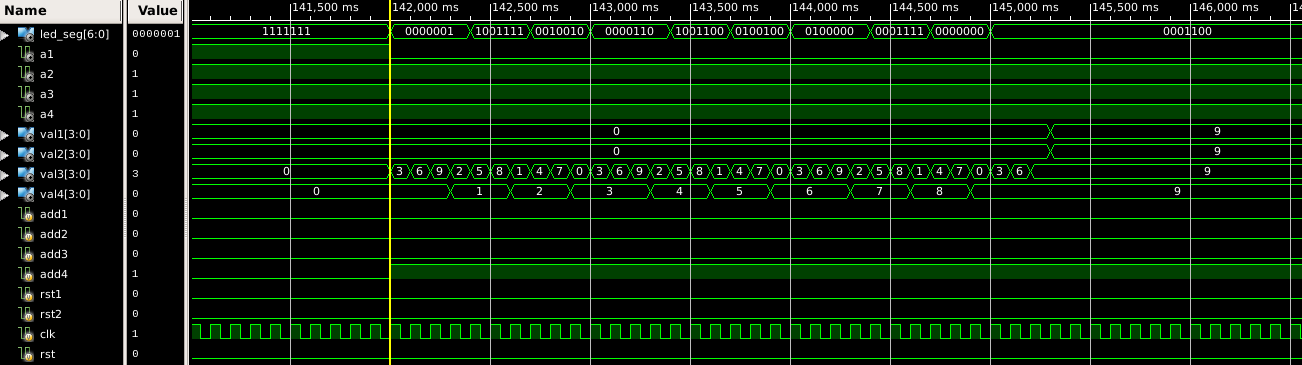
\includegraphics[scale=0.35]{../figs/overflow.png}
            \caption{Testing the maximum display value and over-adding.}
            \label{fig:overflow}
        \end{figure}
\end{enumerate}

\section{Conclusion}
In this project, I successfully implemented a finite state machine for a parking meter. This project was more difficult than it first seemed, but I was able to learn a lot, as well as apply many of the concepts I learned from previous labs into this project.

The most difficult aspect of this project for me was implementing the flashing logic, and making sure that state transitions would react properly to the many different button presses. Writing out all the button functions and drawing out their relations helped tremendously.

Overall, I thought this lab was a great final project for this class. I've learned a lot about practical digital design and how FPGA design works in conjunction with Verilog. From this class, I think programming from a hardware perspective is the skill I gained the most. Thank you Mohit for being a great and supportive TA for all these projects. I really appreciated your prompt and helpful replies to all my questions.

\end{document}